\section{Punto 2}

En este punto se analiza el comportamiento de una señal binaria aleatoria bipolar generada en GNU Radio, evaluando su representación en el dominio del tiempo y su densidad espectral de potencia (PSD). Para ello, se varía el número de muestras por símbolo (Sps) modificando el vector $h$, lo cual permite estudiar el efecto de la interpolación sobre la señal

\subsection{Parámetros principales}

Para todos los casos se mantiene constante la tasa de bits:
\[
R_b = 32 \text{ kbits/s}
\]

Los parámetros principales del sistema se determinan mediante las siguientes relaciones:
\[
F_s = R_b \cdot Sps
\]
\[
T_b = \frac{1}{R_b}
\]
\[
T_s = \frac{1}{F_s}
\]
\[
BW \approx 2R_b = 64 \text{ kHz}
\]
\begin{figure}[t]
    \centering
    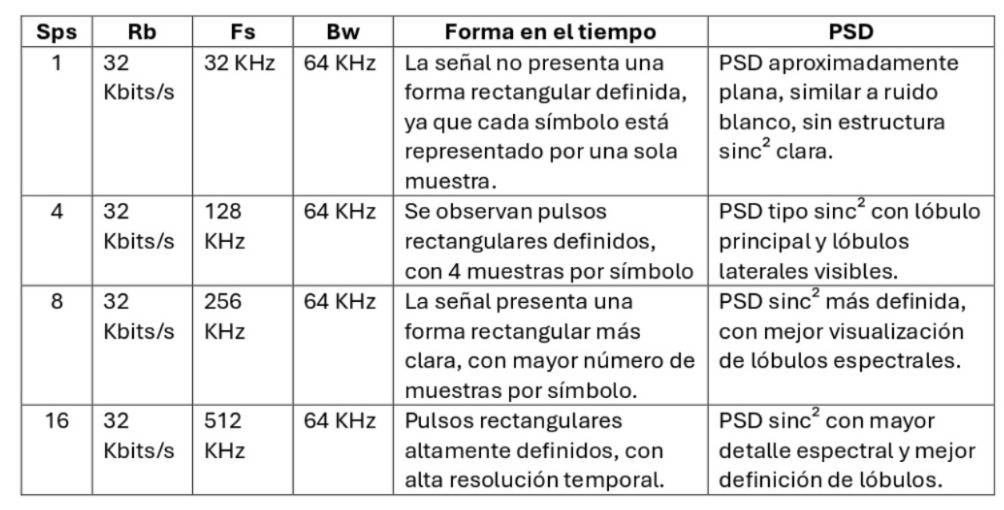
\includegraphics[width=\columnwidth]{imagenes/tab.jpeg}
\end{figure}
\begin{figure}[htbp]
\centering
\begin{subfigure}[b]{0.24\textwidth}
    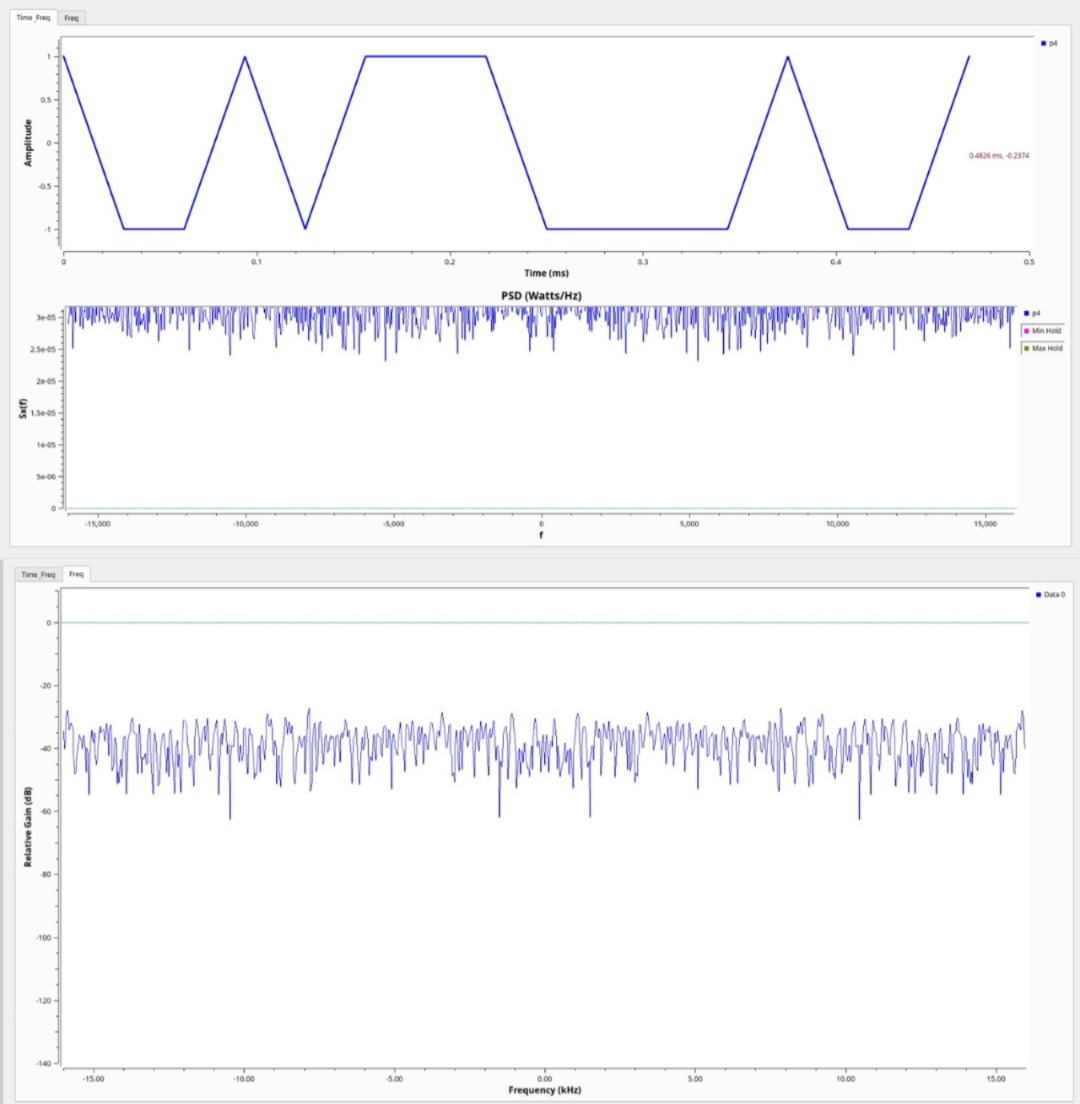
\includegraphics[width=\textwidth]{imagenes/Sps1.jpeg} 
    \caption{Sps = 1}
\end{subfigure}
\hfill
\begin{subfigure}[b]{0.24\textwidth}
    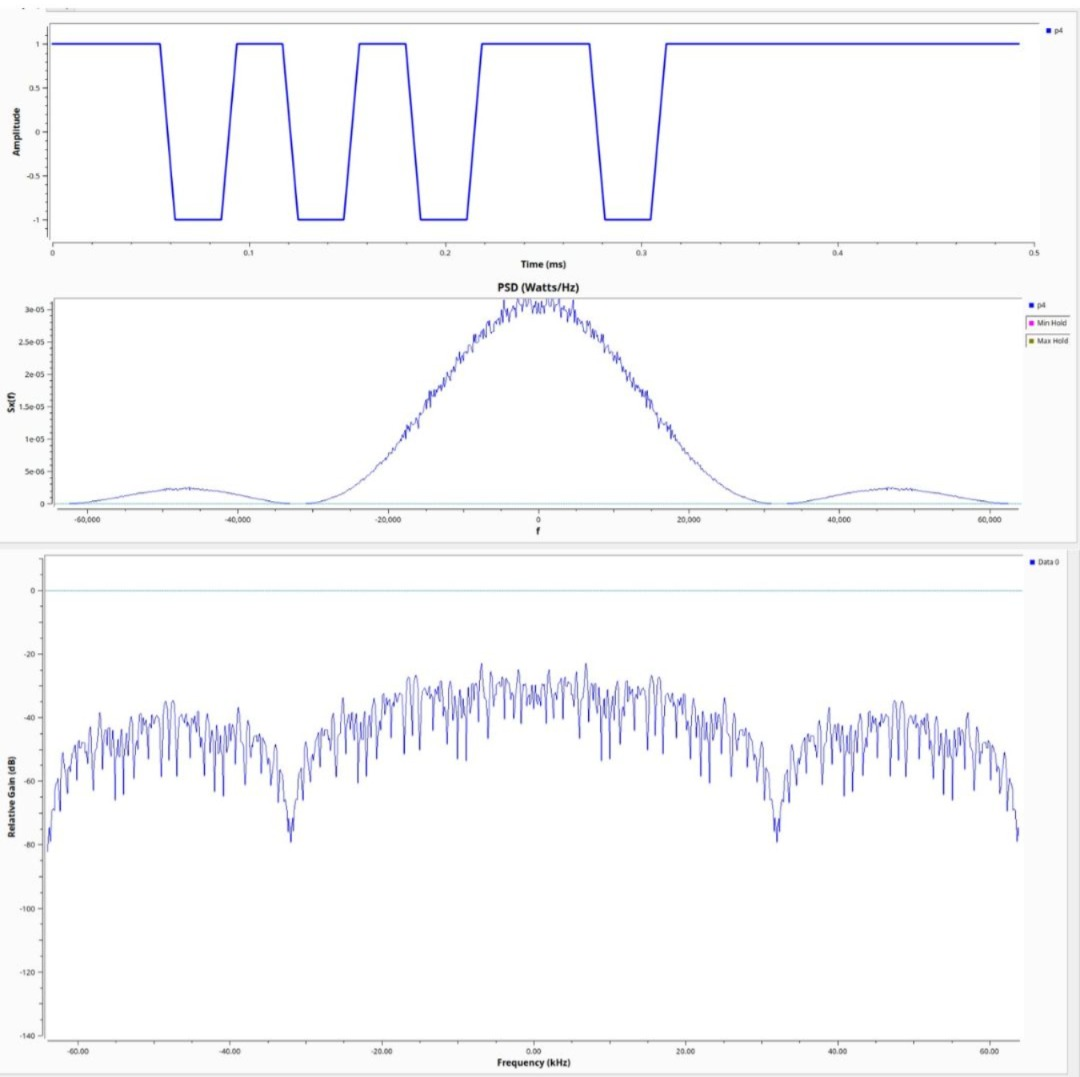
\includegraphics[width=\textwidth]{imagenes/Sps4.jpeg} 
    \caption{Sps = 4}
\end{subfigure}
\end{figure}

\begin{figure}[htbp]
\centering
\begin{subfigure}[b]{0.24\textwidth}
    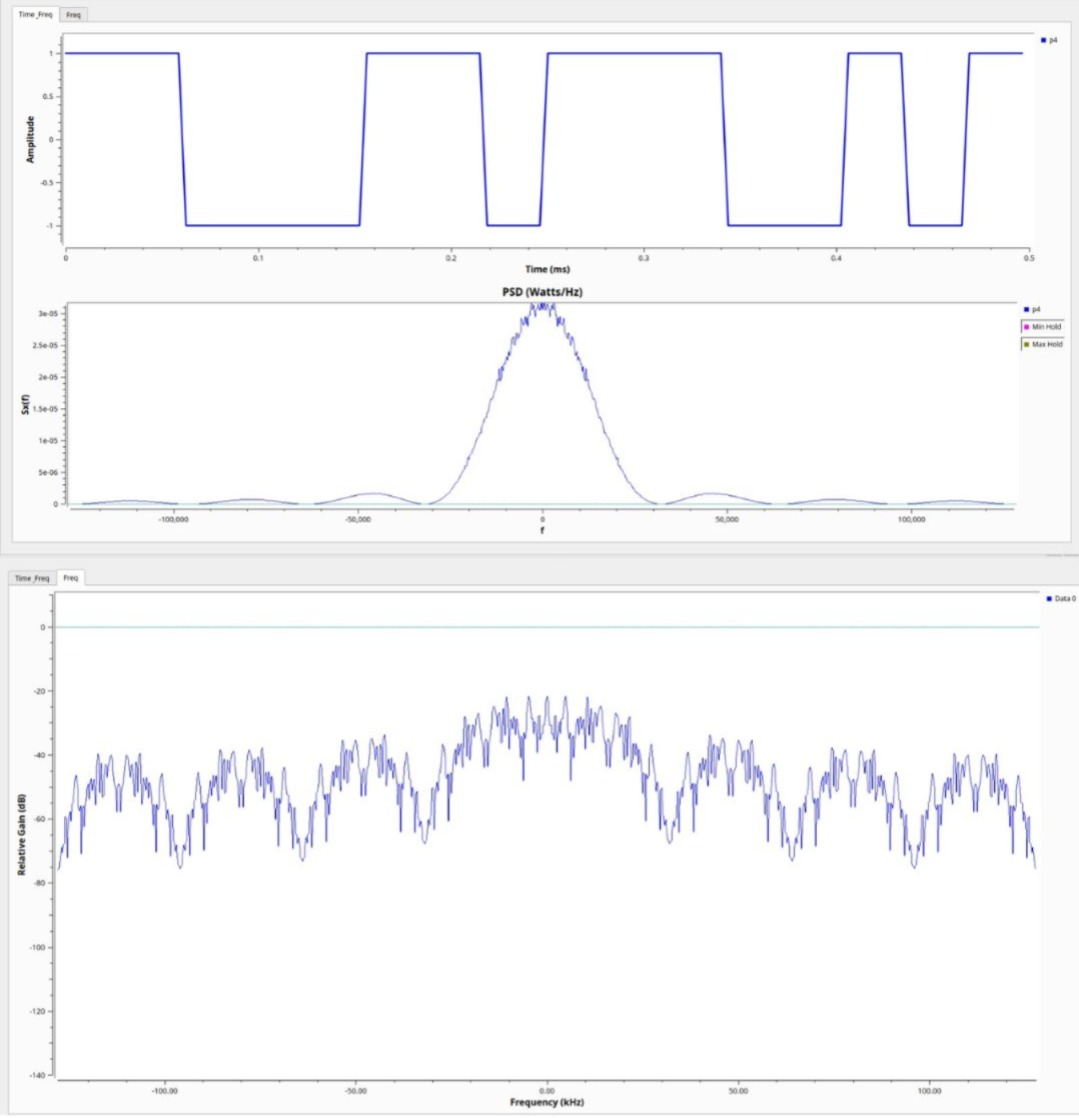
\includegraphics[width=\textwidth]{imagenes/Sps8.jpeg} 
    \caption{Sps = 8}
\end{subfigure}
\hfill
\begin{subfigure}[b]{0.24\textwidth}
    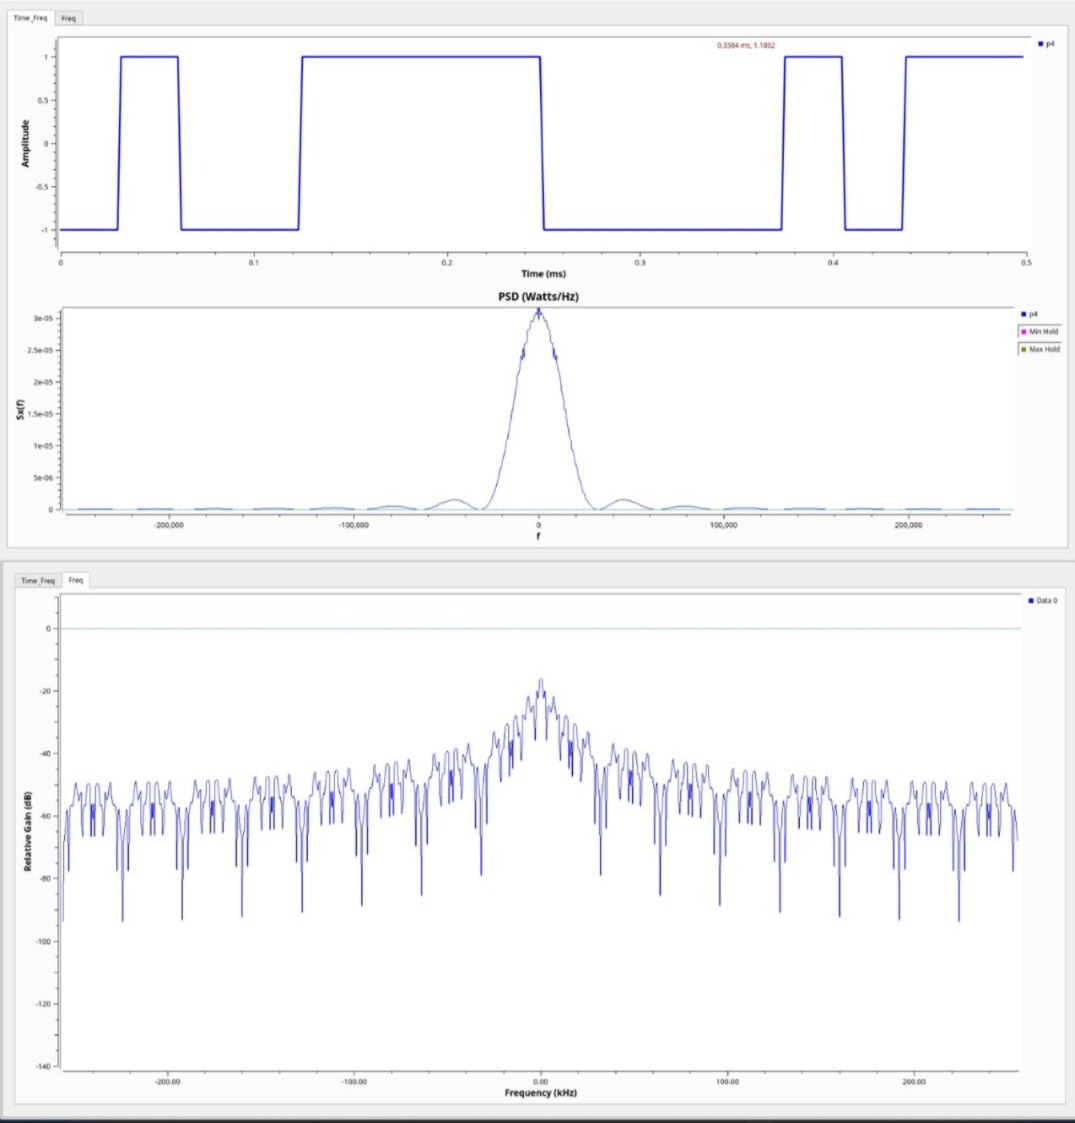
\includegraphics[width=\textwidth]{imagenes/Sps16.jpeg} 
    \caption{Sps = 16}
\end{subfigure}
\end{figure}

\subsection{Análisis de resultados}

Al aumentar el número de muestras por símbolo (Sps), se incrementa la frecuencia de muestreo, lo que mejora la representación de la señal en el dominio del tiempo. Para valores bajos de Sps, como Sps = 1, la señal no presenta una forma de pulso claramente definida, lo que produce una PSD aproximadamente plana similar al ruido.

A medida que Sps aumenta (4, 8 y 16), la señal adquiere una forma rectangular más definida, lo que genera una densidad espectral de potencia con estructura característica tipo sinc$^2$, donde se observan lóbulos laterales y mayor detalle espectral.

El aumento de Sps mejora la resolución temporal y espectral de la señal, permitiendo una mejor visualización de sus características. Sin embargo, el ancho de banda de la señal permanece constante, ya que depende únicamente de la tasa de bits y no del número de muestras por símbolo.

